\documentclass[ngerman,]{article}
\usepackage{lmodern}
\usepackage{amssymb,amsmath}
\usepackage{ifxetex,ifluatex}
\usepackage{fixltx2e} % provides \textsubscript
\ifnum 0\ifxetex 1\fi\ifluatex 1\fi=0 % if pdftex
  \usepackage[T1]{fontenc}
  \usepackage[utf8]{inputenc}
  \usepackage{eurosym}
\else % if luatex or xelatex
  \ifxetex
    \usepackage{mathspec}
  \else
    \usepackage{fontspec}
  \fi
  \defaultfontfeatures{Ligatures=TeX,Scale=MatchLowercase}
  \newcommand{\euro}{€}
\fi
% use upquote if available, for straight quotes in verbatim environments
\IfFileExists{upquote.sty}{\usepackage{upquote}}{}
% use microtype if available
\IfFileExists{microtype.sty}{%
\usepackage{microtype}
\UseMicrotypeSet[protrusion]{basicmath} % disable protrusion for tt fonts
}{}
\usepackage[margin=1in]{geometry}
\usepackage{hyperref}
\hypersetup{unicode=true,
            pdftitle={Wie beeinflusst der Goldene Schnitt die Ziehungswahrscheinlichkeit unter zwei Fibonacci-Zahlen im Lotto 6 aus 49?},
            pdfauthor={Shirin Shahidi, Matrikelnummer 455612},
            pdfborder={0 0 0},
            breaklinks=true}
\urlstyle{same}  % don't use monospace font for urls
\ifnum 0\ifxetex 1\fi\ifluatex 1\fi=0 % if pdftex
  \usepackage[shorthands=off,main=ngerman]{babel}
\else
  \usepackage{polyglossia}
  \setmainlanguage[]{german}
\fi
\usepackage{color}
\usepackage{fancyvrb}
\newcommand{\VerbBar}{|}
\newcommand{\VERB}{\Verb[commandchars=\\\{\}]}
\DefineVerbatimEnvironment{Highlighting}{Verbatim}{commandchars=\\\{\}}
% Add ',fontsize=\small' for more characters per line
\usepackage{framed}
\definecolor{shadecolor}{RGB}{248,248,248}
\newenvironment{Shaded}{\begin{snugshade}}{\end{snugshade}}
\newcommand{\KeywordTok}[1]{\textcolor[rgb]{0.13,0.29,0.53}{\textbf{#1}}}
\newcommand{\DataTypeTok}[1]{\textcolor[rgb]{0.13,0.29,0.53}{#1}}
\newcommand{\DecValTok}[1]{\textcolor[rgb]{0.00,0.00,0.81}{#1}}
\newcommand{\BaseNTok}[1]{\textcolor[rgb]{0.00,0.00,0.81}{#1}}
\newcommand{\FloatTok}[1]{\textcolor[rgb]{0.00,0.00,0.81}{#1}}
\newcommand{\ConstantTok}[1]{\textcolor[rgb]{0.00,0.00,0.00}{#1}}
\newcommand{\CharTok}[1]{\textcolor[rgb]{0.31,0.60,0.02}{#1}}
\newcommand{\SpecialCharTok}[1]{\textcolor[rgb]{0.00,0.00,0.00}{#1}}
\newcommand{\StringTok}[1]{\textcolor[rgb]{0.31,0.60,0.02}{#1}}
\newcommand{\VerbatimStringTok}[1]{\textcolor[rgb]{0.31,0.60,0.02}{#1}}
\newcommand{\SpecialStringTok}[1]{\textcolor[rgb]{0.31,0.60,0.02}{#1}}
\newcommand{\ImportTok}[1]{#1}
\newcommand{\CommentTok}[1]{\textcolor[rgb]{0.56,0.35,0.01}{\textit{#1}}}
\newcommand{\DocumentationTok}[1]{\textcolor[rgb]{0.56,0.35,0.01}{\textbf{\textit{#1}}}}
\newcommand{\AnnotationTok}[1]{\textcolor[rgb]{0.56,0.35,0.01}{\textbf{\textit{#1}}}}
\newcommand{\CommentVarTok}[1]{\textcolor[rgb]{0.56,0.35,0.01}{\textbf{\textit{#1}}}}
\newcommand{\OtherTok}[1]{\textcolor[rgb]{0.56,0.35,0.01}{#1}}
\newcommand{\FunctionTok}[1]{\textcolor[rgb]{0.00,0.00,0.00}{#1}}
\newcommand{\VariableTok}[1]{\textcolor[rgb]{0.00,0.00,0.00}{#1}}
\newcommand{\ControlFlowTok}[1]{\textcolor[rgb]{0.13,0.29,0.53}{\textbf{#1}}}
\newcommand{\OperatorTok}[1]{\textcolor[rgb]{0.81,0.36,0.00}{\textbf{#1}}}
\newcommand{\BuiltInTok}[1]{#1}
\newcommand{\ExtensionTok}[1]{#1}
\newcommand{\PreprocessorTok}[1]{\textcolor[rgb]{0.56,0.35,0.01}{\textit{#1}}}
\newcommand{\AttributeTok}[1]{\textcolor[rgb]{0.77,0.63,0.00}{#1}}
\newcommand{\RegionMarkerTok}[1]{#1}
\newcommand{\InformationTok}[1]{\textcolor[rgb]{0.56,0.35,0.01}{\textbf{\textit{#1}}}}
\newcommand{\WarningTok}[1]{\textcolor[rgb]{0.56,0.35,0.01}{\textbf{\textit{#1}}}}
\newcommand{\AlertTok}[1]{\textcolor[rgb]{0.94,0.16,0.16}{#1}}
\newcommand{\ErrorTok}[1]{\textcolor[rgb]{0.64,0.00,0.00}{\textbf{#1}}}
\newcommand{\NormalTok}[1]{#1}
\usepackage{graphicx,grffile}
\makeatletter
\def\maxwidth{\ifdim\Gin@nat@width>\linewidth\linewidth\else\Gin@nat@width\fi}
\def\maxheight{\ifdim\Gin@nat@height>\textheight\textheight\else\Gin@nat@height\fi}
\makeatother
% Scale images if necessary, so that they will not overflow the page
% margins by default, and it is still possible to overwrite the defaults
% using explicit options in \includegraphics[width, height, ...]{}
\setkeys{Gin}{width=\maxwidth,height=\maxheight,keepaspectratio}
\IfFileExists{parskip.sty}{%
\usepackage{parskip}
}{% else
\setlength{\parindent}{0pt}
\setlength{\parskip}{6pt plus 2pt minus 1pt}
}
\setlength{\emergencystretch}{3em}  % prevent overfull lines
\providecommand{\tightlist}{%
  \setlength{\itemsep}{0pt}\setlength{\parskip}{0pt}}
\setcounter{secnumdepth}{0}
% Redefines (sub)paragraphs to behave more like sections
\ifx\paragraph\undefined\else
\let\oldparagraph\paragraph
\renewcommand{\paragraph}[1]{\oldparagraph{#1}\mbox{}}
\fi
\ifx\subparagraph\undefined\else
\let\oldsubparagraph\subparagraph
\renewcommand{\subparagraph}[1]{\oldsubparagraph{#1}\mbox{}}
\fi

%%% Use protect on footnotes to avoid problems with footnotes in titles
\let\rmarkdownfootnote\footnote%
\def\footnote{\protect\rmarkdownfootnote}

%%% Change title format to be more compact
\usepackage{titling}

% Create subtitle command for use in maketitle
\providecommand{\subtitle}[1]{
  \posttitle{
    \begin{center}\large#1\end{center}
    }
}

\setlength{\droptitle}{-2em}

  \title{Wie beeinflusst der Goldene Schnitt die Ziehungswahrscheinlichkeit unter
zwei Fibonacci-Zahlen im Lotto 6 aus 49?}
    \pretitle{\vspace{\droptitle}\centering\huge}
  \posttitle{\par}
    \author{Shirin Shahidi, Matrikelnummer 455612}
    \preauthor{\centering\large\emph}
  \postauthor{\par}
      \predate{\centering\large\emph}
  \postdate{\par}
    \date{2019-07-20}


\begin{document}
\maketitle

{
\setcounter{tocdepth}{2}
\tableofcontents
}
\newpage

\section{1. Einleitung}\label{einleitung}

``Das, wobei unsere Berechnungen versagen, nennen wir Zufall.'' - Albert
Einstein (zitate.net, 2019, o.S.). Im deutschen Lotto 6 aus 49 lassen
sich Erfolgswahrscheinlichkeiten errechnen, nicht jedoch künftige
Ziehungen vorhersagen. Tendenzen, dass spezifische Ereignisse eintreten,
können auf Basis bereits vergangener Ziehungen statistisch ermittelt
werden (vgl. Ute Sproesser et al., 2014, S.33).

``Etwas hat Gestalt, weil es auf Zahlen beruht{[}\ldots{}{]}'' (Jonak,
2018, S.136). Die menschliche Gestaltwahrnehmung bevorzugt
Vollkommenheit, Symmetrie und bestimmte Proportionen wie etwa den
Goldenen-Schnitt. Diese Wahrnehmungspräferenzen von Gestalten lassen
sich auch im Tierreich beobachten, bei dem Gestaltwahrnehmung instinktiv
zu einer Reaktion führt(vgl. Oerter, 2014, S.252).

Auf Basis dieser Tatsachen stellt sich die Frage, ob die Gestalt der
Lottoziehungen bestimmte Proportionen bevorzugt oder ob Ziehungen
bestimmter Zahlenkombinationen rein zufällig erfolgen. Konzentriert man
sich auf die Proportion des Goldenen Schnittes, so wird dieser gemäß
aktuellem Forschungsstand durch die Formel
\(\frac{\sqrt{5} + 1}{2}\sim1,618\) errechnet (vgl. Kohn, 2019, S.160).
Leonardo of Pisa, auch unter dem Namen Fibonacci bekannt,
veröffentlichte 1202 das Werk \emph{Liber Abbaci}(vgl. Hannah, 2007,
o.S.). In diesem führt er zur Fibonacci-Sequenz hin, welche im Tierreich
die Vermehrung von Hasen in Zahlen beschreibt(vgl. Fibonacci, 1987,
S.18). Im Lotto 6 aus 49 sind die ersten acht Fibonacci-Zahlen
(1,2,3,5,8,13,21,34) enthalten(vgl. Kohn, 2019, S.159). Dividiert man
zwei aufeinander folgende Fibonacci-Zahlen, so konvergieren diese gegen
den Goldene-Schnitt(vgl. Knebl \& Springer Fachmedien Wiesbaden GmbH,
2019, S.29).

Um zur Forschungsfrage hinführen zu können, wird im Folgenden auf die
beliebteste Lotterie namens Lotto 6 aus 49 unter den Einwohnern
Deutschlands eingegangen(vgl. Lotto.de, 2019, o.S.). Spielberechtigt
sind dabei erwachsene Personen ab 18 Jahren, da gemäß Jugendschutzgesetz
§ 6 Spielhallen, Glücksspiele Minderjährigen das Glücksspiel mit Chance
auf hohe Geldbeträge untersagt ist(vgl. JuSchG, 2019, o.S.). Ziel eines
Lottospieles ist es 6 zufällig gezogene Gewinnzahlen aus 1-49 vorgegeben
Ziffern vorherzusagen. Dabei wird ein Lotto-Schein mit 12 möglichen
Tippfeldern und jeweils 49 Zahlen ausgefüllt. Pro Tippfeld werden 6
Zahlen angekreuzt. Jeder Lotto-Schein enthält eine Spielscheinnummer,
deren letzte Ziffer die Superzahl darstellt. Diese Superzahl wird neben
den 6 Gewinnzahlen zufällig aus den Ziffern 0-9 ermittelt. Es müssen
minimal 2 Ziffern und eine Superzahl korrekt prophezeit werden um einen
Gewinn zu erzielen. Der maximale Gewinn stellt 6 richtige Gewinnzahlen
und die korrekte Superzahl dar. Der halbierte Spieleinsatz stellt die
Gewinnsumme dar, welche sich auf 9 Gewinnklassen aufteilen lässt.
Zusätzlich können die Lotterien Spiel 77 und SUPER 6 sowie die
GlücksSpirale im Lotto-Schein ausgewählt werden. Ein Tippfeld im Lotto 6
aus 49 kostet 1,0\euro{} zzgl. Bearbeitungsgebühren. Die Ziehungen
finden wöchentlich mittwochs um 18:25 Uhr und samstags um 19:25 Uhr
unter www.lotto.de statt(vgl. Lotto.de, 2019, o.S.). Die
Wahrscheinlichkeit, zwei konkrete Zahlen im Lotto zu ziehen beträgt
\(1:((\frac{49}{6})*(\frac{48}{5}))\sim0.01276\)(vgl. Lottozahlen.com,
2019, o.S.).

\subsection{1.1. Forschungsfrage}\label{forschungsfrage}

Betrachtet man die bereits genannten Fibonacci Zahlen im Lotto 6 aus 49
und die Konvergenz gegen den Goldenen Schnitt, lässt sich die
Forschungsfrage wie folgt ableiten:

\emph{Wie beeinflusst der Goldene Schnitt die Ziehungswahrscheinlichkeit
unter zwei Fibonacci-Zahlen im Lotto 6 aus 49?}

In einer ersten Hypothese soll geprüft werden, ob eine Fibonacci Zahl
unter allen Fibonacci-Zahlen im Lotto 6 aus 49 am häufigsten mit ihrer
Goldenen-Schnitt Zahl gezogen wird. Im Anschluss daran soll geprüft
werden, ob eine Fibonacci Zahl unter allen Fibonacci-Zahlen im Lotto 6
aus 49 am häufigsten mittwochs mit ihrer Goldenen-Schnitt Zahl gezogen
wird. Dieser Tag wird mit den Samstagsziehungen und den davon
abweichenden Wochentagen verglichen. Die Hypothesen lassen sich wie
folgt formulieren:

\emph{H1: Fibonacci-Zahlen werden unter allen Fibonacci-Zahlen im Lotto
6 aus 49 am häufigsten mit ihrer Goldenen-Schnitt Zahl gezogen}

\emph{H2: Fibonacci-Zahlen werden unter allen Fibonacci-Zahlen im Lotto
6 aus 49 am häufigsten mittwochs mit ihrer Goldenen-Schnitt Zahl
gezogen.}

\subsection{1.2. Ziel der Studie/
Analyse}\label{ziel-der-studie-analyse}

Das Untersuchungsziel der Studie ist deskriptiv ausgerichtet mit der
Anforderung an exakte Ergebnisse und eine repräsentative Stichprobe
sowie der Beschreibung der Grundgesamtheit mit ihren wesentlichen
Merkmalen.(vgl. Kuß, 2012, S.15) Ziel der Studie soll sein,
herauszufinden, ob Fibonacci-Zahlenpaare, die dividiert den
Goldenen-Schnitt ergeben im Lotto 6 aus 49 häufiger zusammen gezogen
werden als Fibonacci-Zahlenpaare ohne den Goldenen-Schnitt Proportionen.
Hierzu sollen nur die Gewinnzahlen ohne Superzahl in Betracht gezogen
wereden, da die Superzahlziehung eine abweichende Wahrscheinlichkeit von
\(\frac{1}{10}\) aufweist. Es werden die Häufigkeiten der
Fibonacci-Zahlen, sowie jeglicher Fibonaccipaar-Ziehungen unter allen
Lotto-Ziehungen von 1955 bis Ende Juni 2019 betrachtet. Sollte sich
herausstellen, dass Zahlenpaare aus dieser Auswahl am häufigsten
zusammen auftreten, so werden diese mit Hilfe der Inferenzstatistik
genauer betrachtet um einen Einfluss des Goldenen-Schnittes auf diese
Zahlenpaare ausfindig machen zu können.

\section{2. Methodik}\label{methodik}

Um die Methodik festlegen zu können, wird auf das Studiendesign, sowie
die Datenerhebung und die angewandten statistsichen Methoden genauer
Bezug genommen (vgl. Kuß, 2012, S.13).

\subsection{2.1. Studiendesign}\label{studiendesign}

Das Studiendesign wird definiert durch die Art der Datenerhebung und
Ziehung der Stichprobe. Die vorliegende Studie basiert auf den
Sekundärforschungen der Westdeutsche Lotterie GmbH \& Co. oHG, sowie den
Datenerhebungen unter www.lottozahlenonline.de durch Gustav Zygmund.
(vgl. Kuß, 2012, S.15)

\subsubsection{2.1.1 Datenerhebung}\label{datenerhebung}

Da es sich um die Beschreibung der Veränderungen der Lotto-Ziehungen im
Zeitablauf von 1955 bis 2019 handelt, wurden die in der Studie
verwendeten Sekundärdaten in Form von Längsschnitt-Untersuchungen als
Beobachtung erhoben. Da das Forschungsproblem auf Basis von
Sekundärdaten bearbeitbar ist, wird in dieser Studie auf die Erhebung
von Primärdaten verzichtet. Die bereits vorhandenen Daten werden für die
Studie neu aufbereitet und analysiert. (vgl. Kuß, 2012, S.16)

\subsubsection{2.1.2 Stichprobe}\label{stichprobe}

Die erhobenen Sekundärdaten stellen alle Ziehungen seit Anbeginn des
Lottos 6 aus 49 von 1955 bis zum Zeitpunkt der Studienanalyse
tabellarisch dar. Werden potenzielle Ungenauigkeiten wie etwa Tipp- oder
Eingabefehler in den bereits vorhandenen Sekundärdaten vernachlässigt,
kann von einer Totalerhebung der Daten ausgegangen werden. Dies führt
dazu, dass Stichprobenfehler die Aussagekraft nicht einschränken
können.(vgl. Kuß, 2012, S.43 f.)

\subsection{2.2 Angewandte statistische
Methoden}\label{angewandte-statistische-methoden}

Um die Daten hinsichtlich ihrer Eignung für statistische Methoden zu
überprüfen, wird eine explorative Datenanalyse zur Verdichtung der Daten
durchgeführt. Da es sich um Häufigkeitsbeobachtungen der
Fibonacci-Zahlenpaare in der Stichprobe handelt, werden Schätzverfahren
angewandt, um Annahmen über entsprechende
Wahrscheinlichkeitsverteilungen in der Grundgesamtheit treffen zu können
(vgl. Kuß, 2012, S.193 f.). Eine Annahme oder Ablehnung der Hypothesen
erfolgt mittels der Zweiseitigen Fragestellung (vgl. Hellbrück, 2009,
S.73--76). Um den Datensatz auf Linearität zu überprüfen wird
anschließend eine lineare Regression durchgeführt (vgl. Hellbrück, 2009,
S.250). Für die Ergebnisse der statistischen Methoden wird die
Programmiersprache R verwendet. Diese ermöglicht den Einsatz moderner
Verfahren der Datenanalyse und ist reproduzierbar, automatisierbar,
quelloffen, kostenlos und grafisch abbildbar. (vgl. Sauer, 2018, S.16
f.) Für den Datensatz wurden die Ergebnisse der Lotto-Ziehungen aus den
Quellen Westdeutsche Lotterie GmbH \& Co. oH

\section{3. Ergebnisse}\label{ergebnisse}

Um zu den Ergebnissen der Studie hinführen zu können werden die bereits
genannten statistischen Methoden im Folgenden anhand von
R-Syntax-Abschnitten (sogenannten Chunks) erklärt, sowie grafisch
veranschaulicht (vgl. Sauer, 2018, S.26).

\subsection{3.1 Kennzahlen der
Stichprobe}\label{kennzahlen-der-stichprobe}

Um einen Überblick über die Kennzahlen der Stichprobe zu erhalten, wird
die Bibliothek ``mosaic'' geladen und der R-Befehl ``inspect''
ausgeführt:

\begin{verbatim}
## 
## categorical variables:  
##        name  class levels    n missing
## 1 Wochentag factor      6 4295       0
##                                    distribution
## 1 Samstag (65.3%), Mittwoch (22.6%) ...        
## 
## quantitative variables:  
##        name   class min Q1 median Q3 max     mean       sd    n missing
## 1 GewZahl_1 integer   1 12     25 37  49 24.64331 14.31717 4295       0
## 2 GewZahl_2 integer   1 12     24 37  49 24.64983 14.25556 4295       0
## 3 GewZahl_3 integer   1 13     25 37  49 25.11665 13.86886 4295       0
## 4 GewZahl_4 integer   1 13     25 37  49 25.06682 13.98750 4295       0
## 5 GewZahl_5 integer   1 13     26 38  49 25.45285 14.06999 4295       0
## 6 GewZahl_6 integer   1 13     26 38  49 25.46123 14.44079 4295       0
\end{verbatim}

Die Stichprobe des Datensatzes Lotto 6 aus 49 von 1955 bis 2019 enthält
6 numerische und eine kategoriale Variable. Insgesamt enthält die
Stichprobe 4295 Beobachtungen. Die numerischen Variablen stellen die
Gewinnzahlen kategorisiert nach Ziehungsrunde dar. Das Minimum liegt bei
der Ziffer 1 und das Maximum bei Ziffer 49. Die kategoriale Variable
nennt den Wochentag, an dem die Beobachtungen aufgezeichnet wurden. Die
Lagemaße und Streumaße sind unterschiedlich ausgeprägt, wie anhand der
Werte von Quantil 1 und 3 sowie der Mittelwerte und dem Median zu
erkennen ist. Die Standardabweichung fällt ebenfalls unterschiedlich
aus. Die Variablennamen werden wie folgt ausgegeben: GewZahl\_1,
GewZahl\_2, GewZahl\_3, GewZahl\_4, GewZahl\_5, GewZahl\_6, Wochentag.
Insgesamt sind keine fehlenden Angaben vorhanden. Einen Überblick über
die letzten 6 Beobachtungen des Datensatzes verschafft der Befehl
``tail'':

\begin{verbatim}
##      GewZahl_1 GewZahl_2 GewZahl_3 GewZahl_4 GewZahl_5 GewZahl_6 Wochentag
## 4290         3        11        15        18        33        45   Samstag
## 4291         3        13        25        27        32        48  Mittwoch
## 4292         5         6        14        16        31        48   Samstag
## 4293         3        22        24        25        43        45  Mittwoch
## 4294         5        14        32        37        46        47   Samstag
## 4295        10        15        31        34        35        45  Mittwoch
\end{verbatim}

\newpage 

\subsection{3.2 explorative Statistik}\label{explorative-statistik}

Anhand der explorativen Statistik sollen Häufigkeitsverteilungen der
Fibonacci-Zahlen betrachtet werden. Hierzu wird der Datensatz nach
Fibonacci-Zahlen mittels R-Skript (``\_01\_Sort\_by\_Fibo.R``) sortiert
und gefiltert. Die daraus gewonnen Daten werden auf
Fibonacci-Zahlenpaare im Goldenen-Schnitt Verhältnis und deren
Häufigkeitsverteilung überprüft und in eine Rangfolge gebracht. Dadurch
zeigt sich, welche Fibonacci-Zahlen mit welcher Fibonacci-Zahl am
häufigsten gemeinsam in einer Ziehung auftreten. Die Rangfolge steigt
von links (seltenste Beobachtung) nach rechts (häufigste Beobachtung)
an:

\begin{Shaded}
\begin{Highlighting}[]
\NormalTok{Fibo_}\DecValTok{1} \CommentTok{#Fibonacci Zahl 1}
\end{Highlighting}
\end{Shaded}

\begin{verbatim}
##   1&13 1&34 1&8 1&5 1&21 1&3 1&2
## 1   44   45  47  54   56  57  59
\end{verbatim}

\begin{Shaded}
\begin{Highlighting}[]
\NormalTok{Fibo_}\DecValTok{2} \CommentTok{#Fibonacci Zahl 2}
\end{Highlighting}
\end{Shaded}

\begin{verbatim}
##   2&13 2&5 2&21 2&3 2&8 2&34 2&1
## 1   42  53   54  55  57   58  59
\end{verbatim}

\begin{Shaded}
\begin{Highlighting}[]
\NormalTok{Fibo_}\DecValTok{3} \CommentTok{#Fibonacci Zahl 3}
\end{Highlighting}
\end{Shaded}

\begin{verbatim}
##   3&8 3&34 3&5 3&2 3&13 3&1 3&21
## 1  48   49  52  55   56  57   57
\end{verbatim}

\begin{Shaded}
\begin{Highlighting}[]
\NormalTok{Fibo_}\DecValTok{5} \CommentTok{#Fibonacci Zahl 5}
\end{Highlighting}
\end{Shaded}

\begin{verbatim}
##   5&34 5&3 2&2 5&1 5&21 5&8 5&13
## 1   45  52  53  54   54  55   57
\end{verbatim}

\begin{Shaded}
\begin{Highlighting}[]
\NormalTok{Fibo_}\DecValTok{8} \CommentTok{#Fibonaci Zahl 8}
\end{Highlighting}
\end{Shaded}

\begin{verbatim}
##   8&13 8&21 8&1 8&3 8&5 8&2 8&34
## 1   38   41  47  48  55  57   57
\end{verbatim}

\begin{Shaded}
\begin{Highlighting}[]
\NormalTok{Fibo_}\DecValTok{13} \CommentTok{#Fibonacci Zahl 13}
\end{Highlighting}
\end{Shaded}

\begin{verbatim}
##   13&8 13&2 13&1 13&34 13&3 13&21 13&5
## 1   38   42   44    47   56    56   57
\end{verbatim}

\begin{Shaded}
\begin{Highlighting}[]
\NormalTok{Fibo_}\DecValTok{21} \CommentTok{#Fibonaci Zahl 21}
\end{Highlighting}
\end{Shaded}

\begin{verbatim}
##   21&8 21&2 21&5 21&13 21&1 21&3 21&34
## 1   41   54   54    56   56   57    63
\end{verbatim}

\begin{Shaded}
\begin{Highlighting}[]
\NormalTok{Fibo_}\DecValTok{34} \CommentTok{#Fibonacci Zahl 34}
\end{Highlighting}
\end{Shaded}

\begin{verbatim}
##   34&5 34&1 34&13 34&3 34&8 34&2 34&21
## 1   45   45    47   49   57   58    63
\end{verbatim}

Aus den Beobachtungen geht hervor, dass die Fibonacci-Zahlen 1, 2, 21
und 34 am häufigsten mit ihren goldenen Schnitt Zahlen gezogen wurden.
Daraus ergibt sich die erste Hypothese: Die Fibonacci-Zahlen 1,2,21 und
34 werden im Lotto 6 aus 49 am häufigsten mit ihrer goldenen Schnitt
Zahl gezogen.

Die Verteilung der Wochentage im Lotto lässt sich anhand Abbildung 1
veranschaulichen. Betrachtet man die Häufigkeitsverteilung der
Fibonacci-Zahlenpaare 1\&2 sowie 21\&34 hinsichtlich der Wochentage
ergibt sich Abbildung 2.Aus diesen Beobachtungen lässt sich die Hyothese
ableiten, dass die Fibonacci Zahlen 1,2,21 und 34 samstags am häufigsten
mit ihren Goldenen-Schnitt Zahlen gezogen werden.

\begin{figure}

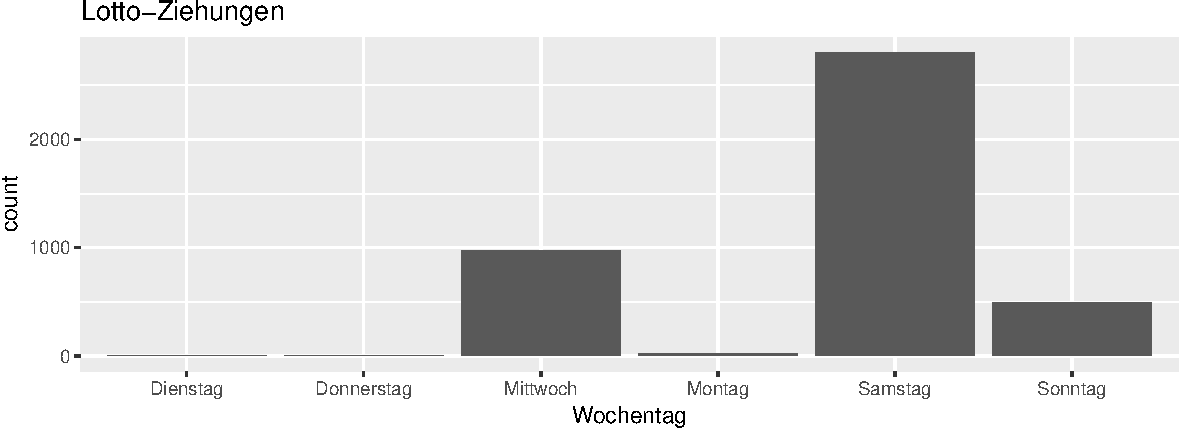
\includegraphics{Abbildung/unnamed-chunk-2-1} \hfill{}

\caption{Die Lotto-Ziehungen von 1955 bis 2019 fanden am häufigsten samstags statt.}\label{fig:unnamed-chunk-2}
\end{figure}

\begin{figure}

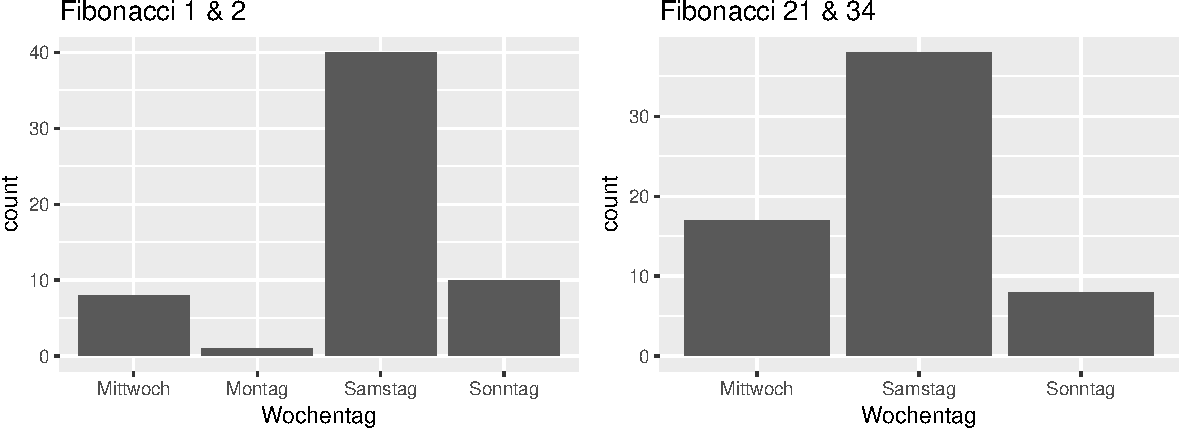
\includegraphics{Abbildung/unnamed-chunk-3-1} \hfill{}

\caption{Die Fibonacci Zahlen 1,2,21 und 34 werden samstags am häufigsten mit ihrer Goldenen-Schnitt Zahlen gezogen.}\label{fig:unnamed-chunk-3}
\end{figure}

\newline
Die relativen Häufigkeitsverteilungen ergebn sich anhand folgender
R-Befehle:

\begin{Shaded}
\begin{Highlighting}[]
\CommentTok{#relative Häufigkeit Ziehungen Fibonacci-Zahlenpaar 1&2 in Prozent}
\NormalTok{(}\DecValTok{59}\OperatorTok{/}\DecValTok{4295}\NormalTok{)}\OperatorTok{*}\DecValTok{100}
\end{Highlighting}
\end{Shaded}

\begin{verbatim}
## [1] 1.37369
\end{verbatim}

\begin{Shaded}
\begin{Highlighting}[]
\CommentTok{#relative Häufigkeit Ziehungen Fibonacci-Zahlenpaar 21&34 in Prozent}
\NormalTok{(}\DecValTok{63}\OperatorTok{/}\DecValTok{4295}\NormalTok{)}\OperatorTok{*}\DecValTok{100}
\end{Highlighting}
\end{Shaded}

\begin{verbatim}
## [1] 1.466822
\end{verbatim}

\begin{Shaded}
\begin{Highlighting}[]
\CommentTok{#absolute Anzahl Ziehungen Fibonacci-Zahlenpaar 1&2 samstags}
\NormalTok{Fibo1_2sa <-}\StringTok{ }\NormalTok{Fibo1_}\DecValTok{2}\OperatorTok\KeywordTok{filter}\NormalTok{(Wochentag}\OperatorTok{==}\StringTok{"Samstag"}\NormalTok{)}
\CommentTok{#absolute Anzahl Ziehungen samstags}
\NormalTok{Lotto_sa <-}\StringTok{ }\NormalTok{data_lotto_orig }\OperatorTok\StringTok{ }\KeywordTok{filter}\NormalTok{(Wochentag}\OperatorTok{==}\StringTok{"Samstag"}\NormalTok{)}
\CommentTok{#relative Anzahl Ziehungen Fibonacci-Zahlenpaar 1&2 samstags in Prozent}
\NormalTok{(}\KeywordTok{nrow}\NormalTok{(Fibo1_2sa)}\OperatorTok{/}\KeywordTok{nrow}\NormalTok{(Lotto_sa))}\OperatorTok{*}\DecValTok{100}
\end{Highlighting}
\end{Shaded}

\begin{verbatim}
## [1] 1.426025
\end{verbatim}

\newpage 

\subsection{3.3 deskriptive Statistik}\label{deskriptive-statistik}

\subsection{3.4 Inferenzstatistik}\label{inferenzstatistik}

\subsubsection{3.4.1 Bootstrap}\label{bootstrap}

\subsubsection{3.4.2 Permutation}\label{permutation}

\subsubsection{3.4.3 Lineare Regression}\label{lineare-regression}

Gehen Sie hier näher auf die \emph{verwendeten} Variablen ein. In R
markdown Dateien können Sie einfach den R Code in Chunks einfügen
(sogenannte ``Code Chunks''). Entweder über das Menü
\texttt{Insert\ -\textgreater{}\ R} oder über die Tastenkombination
\texttt{strg+alt+i}.

Hier stellen und beschreiben Sie die Ergebnisse Ihrer kleinen Studie.
Ihre Ergebnisse stellen Sie graphisch und/ oder tabellarisch dar. Ganz
allgemein wird im Resultateteil NICHT interpretiert, sondern die
Ergebnisse ausschließlich beschrieben.

Der Ergebnisteil kann zur besseren Orientierung und zum besseren Lesen
weitere Gliederungspunkte enthalten (z.B. bei Hypothesenwechsel, für
jedes Ergebnis o.ä.).

\begin{itemize}
\tightlist
\item
  die Abbildungen werden durchnummeriert (Abbildung 1 bis Abbildung xx)
  ebenso die Tabellen.
\item
  Jede Abbildung erhält eine Bildunterschrift und jede Tabelle eine
  Beschreibung (über der Tabelle).
\item
  die Bildunterschrift dürfen Sie mit R markdown machen oder aber in
  word! Eine Vorlage für eine Bildunterschrift ist im Template
  enthalten.
\end{itemize}

Beispiel für Ergebisbeschreibung und einer Figure caption =
Bildunterschrift:

Die Ergebnisse graphisch und tabellarisch dargestellt. Eine
tabellarische Darstellung der Ergebnisse ist im Teil der deskriptiven
Statistik oft sinnvoll. Sie entscheiden hier was eine sinnvolle
Darstellung ist!

 Beschreiben Sie das zentrale Ergebnis und Auffälligkeiten.

\textbf{Folgendes sollte im Ergebnisteil enthalten/ ver- oder
beararbeitet sein: } 1. Kennzahlen 2. explorative / deskriptive
Statistik 3. Inferenzstatistik

Beschreiben Sie Ihre Stichprobe und Ihre Variablen. Das ist hilfreich
zum Verständnis und Nachvollziehbarkeit Ihrer Studie, der Datenerhebung
und der Hypothesentestung.

Gehen Sie hier genauer auf die untersuchten Hypothesen und Modelle ein.
Geben Sie zur Methodik 1-3 Literaturquellen an.

\section{4. Diskussion}\label{diskussion}

Für die Diskussion setzen Sie das Ergebnis in Kontext zu bereits
publizierter Literatur! (hier ist das Lesen und die Angabe (CAVE:
richtig zitieren) von Literatur notwendig) Mind. 3 Literaturquellen

\section{5. Schlussfolgerungen}\label{schlussfolgerungen}

``Es steckt oft mehr Geist und Scharfsinn in einem Irrtum als in einer
Entdeckung.'' - Joseph Joubert

Fassen Sie hier kurz die zentralen Ergebnisse für Ihre
Forschungsthematik zusammen. Gehen Sie auch auf die Grenzen Ihrer
Analyse ein.

\section{Literaturverzeichnis}\label{literaturverzeichnis}

Hier stehen die im Text verwendeten Quellen:

\begin{itemize}
\tightlist
\item
  Nachname Autor1, Anfangsbuchstabe Vorname Autor1, Nachname Autor2,
  Anfangsbuchstabe Vorname Autor2 1 \& Nachname Autor3, Anfangsbuchstabe
  Vorname Autor3, \ldots{} (Jahr der Veröffentlichung). Titel des
  Beitrags. Journal, Volume, Issue, Seitenzahlen
\end{itemize}

\hypertarget{refs}{}
\hypertarget{ref-fibonacci_introduction:_1987}{}
Fibonacci, L.P. (1987) INTRODUCTION: A Brief Biography of Leonardo
Pisano (Fibonacci) {[}1170-post 1240{]}. In: LEONARDO PISANO Fibonacci
(Hrsg.). \emph{The Book of Squares}. {[}Online{]}. San Diego, Academic
Press. S. xv--xx. Available from:
doi:\href{https://doi.org/10.1016/B978-0-08-088650-3.50005-0}{10.1016/B978-0-08-088650-3.50005-0}
{[}Zugegriffen: 15 Juli 2019{]}.

\hypertarget{ref-hannah_false_2007}{}
Hannah, J. (2007) False position in Leonardo of Pisa's Liber Abbaci.
\emph{Historia Mathematica}. {[}Online{]} 34 (3), 306--332. Available
from:
doi:\href{https://doi.org/10.1016/j.hm.2006.10.004}{10.1016/j.hm.2006.10.004}
{[}Zugegriffen: 15 Juli 2019{]}.

\hypertarget{ref-hellbruck_angewandte_2009}{}
Hellbrück, R.P. (2009) OCLC: 458747755. \emph{Angewandte Statistik mit
R: eine Einführung für Ökonomen und Sozialwissenschaftler}. Lehrbuch. 1.
Aufl. Wiesbaden, Gabler.

\hypertarget{ref-jonak_essays_2018}{}
Jonak, U. (2018) \emph{Essays zur Architektur}. {[}Online{]}. Wiesbaden,
Springer Fachmedien Wiesbaden. Available from:
doi:\href{https://doi.org/10.1007/978-3-658-19129-0}{10.1007/978-3-658-19129-0}
{[}Zugegriffen: 8 Juli 2019{]}.

\hypertarget{ref-juschg_juschg_2019}{}
JuSchG (2019) \emph{JuSchG - Jugendschutzgesetz}. {[}Online{]}. 2019.
Available from:
\url{https://www.gesetze-im-internet.de/juschg/BJNR273000002.html}
{[}Zugegriffen: 16 Juli 2019{]}.

\hypertarget{ref-knebl_algorithmen_2019}{}
Knebl, H. \& Springer Fachmedien Wiesbaden GmbH (2019) OCLC: 1098316960.
\emph{Algorithmen und Datenstrukturen Grundlagen und probabilistische
Methoden für den Entwurf und die Analyse}.

\hypertarget{ref-kohn_mathematik_2019}{}
Kohn, W. (2019) OCLC: 1102475595. \emph{MATHEMATIK FR
WIRTSCHAFTSINFORMATIKER: grundlagen und anwendungen.} S.l., SPRINGER.

\hypertarget{ref-kus_marktforschung:_2012}{}
Kuß, A. (2012) OCLC: 795116334. \emph{Marktforschung: Grundlagen der
Datenerhebung und Datenanalyse}. Springer-Gabler-Lehrbuch. 4., überarb.
Aufl. Wiesbaden, Springer Gabler.

\hypertarget{ref-lotto.de_lotto_2019}{}
Lotto.de (2019) \emph{LOTTO 6aus49 Spielregeln LOTTO.de}. {[}Online{]}.
2019. Available from:
\url{https://www.lotto.de/lotto-6aus49/spielregeln} {[}Zugegriffen: 16
Juli 2019{]}.

\hypertarget{ref-lottozahlen.com_6_2019}{}
Lottozahlen.com (2019) \emph{6 aus 49 Wahrscheinlichkeit einfach
erklärt. Lottozahlen}. {[}Online{]}. 2019. Available from:
\url{https://www.lottozahlen.com/lotto-nachrichten/6-aus-49-wahrscheinlichkeit-einfach-erklaert}
{[}Zugegriffen: 16 Juli 2019{]}.

\hypertarget{ref-oerter_mensch_2014}{}
Oerter, R. (2014) OCLC: 887522626. \emph{Der Mensch, das wundersame
Wesen: was Evolution, Kultur und Ontogenese aus uns machen}. Wiesbaden,
Springer Spektrum.

\hypertarget{ref-sauer_moderne_2018}{}
Sauer, S. (2018) \emph{Moderne Datenanalyse mit R: Daten einlesen,
aufbereiten, visualisieren und modellieren}. FOM-Edition. 1. Auflage
2019. Wiesbaden, Springer Fachmedien Wiesbaden GmbH.

\hypertarget{ref-ute_sproesser_et_al._daten_2014}{}
Ute Sproesser et al. (2014) \emph{Daten, Zufall und der Rest der Welt:
didaktische Perspektiven zur anwendungsbezogenen Mathematik}. Research.
Silvia Wessolowski \& Claudia Wörn (Hrsg.). Wiesbaden, Springer
Spektrum.

\hypertarget{ref-zitate.net_zufallzitate_2019}{}
zitate.net (2019) \emph{Zufallzitate Top 20 Zitate und Sprüche über
Zufälle ... Zitate.net}. {[}Online{]}. 2019. Available from:
\url{http://zitate.net/zufall-zitate} {[}Zugegriffen: 14 Juli 2019{]}.


\end{document}
